\documentclass[11pt,a4paper]{article}
\usepackage[margin=1in]{geometry}
\usepackage[T1]{fontenc}
\usepackage[utf8]{inputenc}
\usepackage{lmodern}
\usepackage{microtype}
\usepackage{amsthm,amsmath,amssymb,amsfonts}
\usepackage{mathtools}
\usepackage{booktabs}
\usepackage{ifthen}
\usepackage{tikz}
\usepackage[colorlinks,urlcolor=blue!50!black,linkcolor=blue!50!black,citecolor=green!40!black]{hyperref}
\usepackage{cleveref}

\newtheorem{theorem}{Theorem}
\newtheorem{lemma}{Lemma}
\newtheorem{observation}{Observation}
\theoremstyle{definition}
\newtheorem{definition}{Definition}
\newtheorem{construction}{Construction}
\crefname{construction}{Construction}{Constructions}
\Crefname{construction}{Construction}{Constructions}
\crefname{observation}{Observation}{Observations}
\Crefname{observation}{Observation}{Observations}

\newcommand{\doi}[1]{DOI: \href{https://doi.org/#1}{\nolinkurl{#1}}}
\newcommand{\pmax}{p_{\max}}
\newcommand{\ProbEM}{\textsc{Interval Scheduling on Eligible Machines}}
\newcommand{\MCC}{\textsc{Multicolored Clique}}
\newcommand{\SAT}{\textsc{(3,4)-SAT}}
\newcommand{\bigO}{O}
\newcommand{\FPT}{\textnormal{\textsf{FPT}}}
\newcommand{\Wone}{\textnormal{\textsf{W[1]}}}
\newcommand{\NP}{\textnormal{\textsf{NP}}}

\title{On the Parameterized Complexity of Interval Scheduling\\ with Eligible Machine Sets, formalized}
\author{Yuval Itzhaki \and Claude}
\date{}

\begin{document}
\maketitle

\begin{abstract}
In \ProbEM, a set of $n$ jobs is to be processed non-preemptively on a set of $m$ machines.
Each job has a processing time, a deadline, a weight, and a set of eligible machines that
can process it. The goal is to find a maximum weight subset of jobs that can each be
processed on one of its eligible machines such that it completes exactly at its deadline.
Hermelin, Itzhaki, Molter and Shabtay~\cite{HIMS24} showed that the problem is \Wone-hard
when parameterized by the number $m$ of machines, \NP-hard even when the largest processing
time $\pmax$ is constant, and fixed-parameter tractable for the combined parameter
$m+\pmax$. All three results are proved in Lean. This note presents the definitions,
constructions and statements as they are formalized, in the notation of~\cite{HIMS24}, and
links each of them to its Lean counterpart.
\end{abstract}

\section{Introduction}

In an interval scheduling problem each job can be processed only in a fixed time interval,
and a schedule only decides which machine processes it. In \ProbEM\ every job $j$ comes
with a set $M_j$ of eligible machines. Arkin and Silverberg~\cite{AS87} showed that the
problem is strongly \NP-hard and solvable in $\bigO(n^{m+1})$ time, and whether it is
fixed-parameter tractable for $m$ was Open Problem~8 in the list of Mnich and van
Bevern~\cite{MvB18}. The paper~\cite{HIMS24} answers this question negatively
(\Cref{thm:w1hard}), shows that a constant $\pmax$ does not help either (\Cref{thm:nph}),
and gives an algorithm for the combination of both parameters (\Cref{thm:fpt}).

% lax begin lax-808846
Running times are stated on the word RAM: a program is a fixed list of instructions
operating on words of $w$ bits, and its running time is the number of instructions it
executes. A statement about a running time is a statement about one program, at every word
length that admits the input.
% lax end

\section{Preliminaries}\label{sec:0}

% lax begin Lax470956.Scheduling
\begin{definition}[\ProbEM]
We have a set of $n$ jobs $\{j_1,\ldots,j_n\}$ and a set of $m$ machines
$\{i_1,\ldots,i_m\}$, each of which can process one job at a time. Every job $j$ has a
processing time $p_j\ge 1$, a deadline $d_j\ge p_j$, a weight $w_j$, and a set of eligible
machines $M_j\subseteq\{i_1,\ldots,i_m\}$. Job $j$ can be processed only in the interval
$[d_j-p_j,d_j)$. We denote the largest processing time by $\pmax=\max_{1\le j\le n}p_j$.

A \emph{schedule} is a function $\sigma:\{j_1,\ldots,j_n\}\to\{i_1,\ldots,i_m,\bot\}$ with
$\sigma(j)\in M_j\cup\{\bot\}$; job $j$ is scheduled on machine $\sigma(j)$, or not
scheduled if $\sigma(j)=\bot$. Two jobs $j,j'$ are \emph{in conflict} if
$[d_j-p_j,d_j)\cap[d_{j'}-p_{j'},d_{j'})\neq\emptyset$. A schedule $\sigma$ is
\emph{feasible} if there is no pair of conflicting jobs $j,j'$ with
$\sigma(j)=\sigma(j')\neq\bot$. Its weight is $w(\sigma)=\sum_{\sigma(j)\neq\bot}w_j$.
The goal is to find a feasible schedule of maximum weight.
\end{definition}
% lax end

% lax begin Lax470956.InstanceEncoding
An instance is given to a word RAM as a word of numbers: $n$, $m$, the processing times,
the deadlines, the weights, and the sets $M_j$ as $n+1$ offsets into one array that lists
the eligible machines of each job in turn. In the decision version the word ends with the
target weight $W$.
% lax end
% lax begin Lax470956.BinaryEncoding
For \NP-hardness an instance is encoded as a binary word, with the sets $M_j$ as an
$n\times m$ matrix.
% lax end

% lax begin Lax470956.SchedulingProblems
We consider three problems on these words: deciding whether there is a feasible schedule
$\sigma$ with $w(\sigma)\ge W$, parameterized by $m$; the same problem parameterized by
$m+\pmax$; and deciding whether there is a feasible schedule in which all jobs are
scheduled, parameterized by $\pmax$.
% lax end

% lax begin Lax470956.ParameterizedComplexity
\begin{definition}[\FPT\ and parameterized reductions]
A parameterized problem is \emph{fixed-parameter tractable} if there are a program, a
constant $c$ and a function $g$ such that the program decides every input $x$ with
parameter $k$ within $c\cdot g(k)\cdot(|x|+1)$ instructions. A \emph{parameterized
reduction} from a problem $P$ to a problem $Q$ is a function on words that is computed by a
program within such a bound, maps yes-instances to yes-instances and no-instances to
no-instances, and maps an input with parameter $k$ to one with parameter at most $h(k)$
for some function $h$.
\end{definition}
The bound is linear in $|x|$, where $f(k)\cdot|x|^{\bigO(1)}$ is usually allowed, so a
problem that is fixed-parameter tractable in this sense is so in the usual sense, and a
parameterized reduction in this sense is one in the usual sense.
% lax end

% lax begin Lax470956.NPHardness
\begin{definition}[\NP-hardness on a class of instances]
A scheduling problem is \emph{\NP-hard} if every language in \NP\ has a polynomial-time
many-one reduction to it. It is \emph{\NP-hard on a class} $\mathcal{C}$ of instances if
the reductions can be chosen to produce only instances in $\mathcal{C}$.
\end{definition}
% lax end
% lax begin Lax470956.PolynomialReduction
The reductions we construct are computed by word RAM programs in time polynomial in the
number of bits of the input, which is polynomial time on a Turing machine.
% lax end

\section{\textsf{W[1]}-hardness for number \texorpdfstring{$\boldsymbol{m}$}{m} of machines}\label{sec:1}

% lax begin Lax470956.MulticolouredClique
\begin{definition}[\MCC]
We are given a $k$-partite graph $G=(V_0\uplus V_1\uplus\ldots\uplus V_{k-1},E)$ and are
asked whether $G$ contains a clique of size $k$. The $k$ vertex parts are called
\emph{colors}, and the parameter is $k$.
\end{definition}
% lax end
\MCC\ parameterized by $k$ is \Wone-hard~\cite{FHRV09}.

% lax begin Lax470956.Construction1
\begin{construction}\label{const:w1hard}
Let $G=(V_0\uplus V_1\uplus\ldots\uplus V_{k-1},E)$ be a $k$-partite graph with $n_G$
vertices. Let $<_\pi$ be the total ordering of $V:=V_0\uplus\ldots\uplus V_{k-1}$ that
orders the vertices by color and breaks ties by index, so that $u<_\pi v$ whenever
$u\in V_\ell$, $v\in V_{\ell'}$ and $\ell<\ell'$. Let $\pi(v)\in\{1,\ldots,n_G\}$ denote the
ordinal position of $v$ in $<_\pi$. Let $c_1=n_G+1$, $c_2=(k-1)n_Gc_1+n_G+1$, and
$c_3=(kn_G+k^2n_G)n_Gc_2+1$.

We create $m=\binom{k}{2}+1$ machines: one \emph{edge selection machine} for each color
combination $\ell,\ell'$ with $\ell<\ell'$, and one \emph{validation machine}. We create
the following jobs.
\begin{itemize}
\item For each vertex $v\in V_\ell$ we create $k$ \emph{vertex jobs} $j_v^{(0)},\ldots,j_v^{(k-1)}$.
  The job $j_v^{(\ell)}$ has processing time $k+2$, deadline $(k+2)\pi(v)+1$ and weight $1$.
  For each color $\ell'\neq\ell$ the job $j_v^{(\ell')}$ has processing time $1$, deadline
  $(k+2)\pi(v)-\ell'$ and weight $c_1$.
\item For each edge $e=\{u,v\}\in E$ with $u\in V_\ell$, $v\in V_{\ell'}$ and $\ell<\ell'$ we
  create one \emph{edge job} $j_e$ with processing time $(k+2)(\pi(v)-\pi(u))-\ell+\ell'-1$,
  deadline $(k+2)\pi(v)-\ell-1$ and weight $c_2(\pi(v)-\pi(u))+c_3$.
\item For each color combination $\ell<\ell'$ we create $|V_\ell|+|V_{\ell'}|$ \emph{color
  combination jobs}. For $u\in V_\ell$ the job $j_u^{(\ell,\ell')}$ has processing time
  $(k+2)\pi(u)-\ell'-2$, deadline $(k+2)\pi(u)-\ell'-1$ and weight $c_2\pi(u)$. For
  $v\in V_{\ell'}$ the job $j_v^{(\ell,\ell')}$ has processing time
  $(k+2)(n_G-\pi(v))+\ell+2$, deadline $(k+2)n_G+2$ and weight $c_2(n_G-\pi(v))$.
\end{itemize}
The validation machine is an eligible machine of all vertex jobs. The edge selection
machine for color combination $\ell,\ell'$ with $\ell<\ell'$ is a further eligible machine
of the vertex jobs $j_u^{(\ell')}$ with $u\in V_\ell$ and $j_v^{(\ell)}$ with
$v\in V_{\ell'}$, and it is the only eligible machine of the color combination jobs
$j_u^{(\ell,\ell')}$, $j_v^{(\ell,\ell')}$ and of the edge jobs $j_e$ with $e=\{u,v\}$,
$u\in V_\ell$ and $v\in V_{\ell'}$. The target weight is
\[
W=\binom{k}{2}c_3+\binom{k}{2}n_Gc_2+(k-1)n_Gc_1+k.
\]
\end{construction}
Two details are done slightly differently than in~\cite{HIMS24}: the colors are numbered
from $0$, and the processing time of an edge job is one unit shorter. On the edge
selection machine for $\ell,\ell'$ the jobs $j_u^{(\ell,\ell')}$, $j_u^{(\ell')}$, $j_e$,
$j_v^{(\ell)}$ and $j_v^{(\ell,\ell')}$ then have consecutive intervals, as illustrated in
\Cref{fig:w1_edge_selection,fig:w1_overview}.
% lax end

\begin{figure}[tb]
    \centering
    % The edge selection machine of a color combination (Figure 1 of the paper).
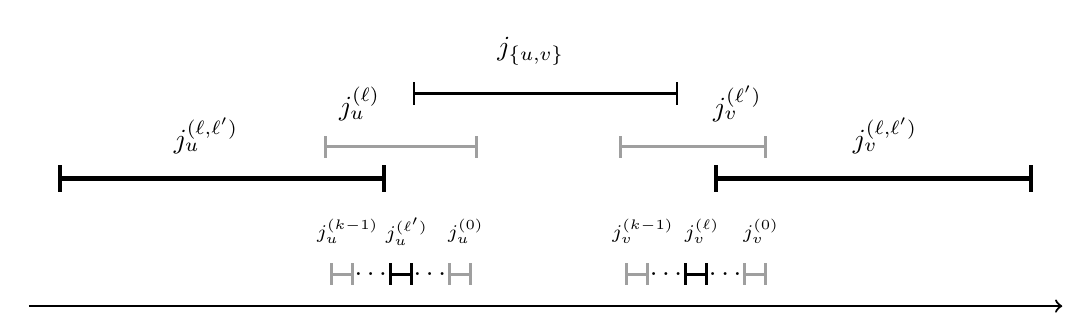
\begin{tikzpicture}[scale=0.75,yscale=1.8]
\def\eps{0.1}
\def\shiftx{5}
\colorlet{grayed}{gray!75}

    \draw[thick,->] (0,0) -- (17.5,0);

    \draw[line width=1.5, |-|] ({0.5}, 1.2) -- (6.05, 1.2);
    \node at (3, 1.6) {$j_u^{(\ell,\ell')}$};

    \draw[line width=1.5, |-|] ({\shiftx+6.6}, 1.2) -- (7+\shiftx+5, 1.2);
    \node at (\shiftx+7+2.5, 1.6) {$j_v^{(\ell,\ell')}$};

    % the vertex jobs of u
    \draw[line width=1,grayed, |-|] (5, 1.5) -- (7.6, 1.5);
    \node at (5.6, 1.9) {$j_u^{(\ell)}$};
    \foreach \x\i\label in {0/1/$j_u^{(k-1)}$, 1/2/$ $, 2/3/$j_u^{(\ell')}$, 3/4/$ $, 4/5/$j_u^{(0)}$}
    {
        \ifthenelse{\(\i=2 \OR \i=4\)}
        {
            \node at (\eps+5+2*\x/5+\eps*\x+0.23, 0.3) {$\dots$};
        }
        {
            \ifthenelse{\(\NOT \i=3\)}
            {
            \draw[line width=1, grayed, |-|]
            (\eps+5+2*\x/5+\eps*\x, 0.3) -- (\eps+5+2*\x/5+0.4+\eps*\x, 0.3);
            \node at (\eps+5+2*\x/5+\eps*\x+0.3, 0.7) {\scriptsize\label};
            }
            {
            \draw[line width=1, |-|]
            (\eps+5+2*\x/5+\eps*\x, 0.3) -- (\eps+5+2*\x/5+0.4+\eps*\x, 0.3);
            \node at (\eps+5+2*\x/5+\eps*\x+0.3, 0.7) {\scriptsize\label};
            }
        }
    }

    % the vertex jobs of v
    \draw[line width=1,grayed, |-|] (5+\shiftx, 1.5) -- (7.5+\shiftx, 1.5);
    \node at (7.0+\shiftx, 1.9) {$j_v^{(\ell')}$};
    \foreach \x\i\label in {0/1/$j_v^{(k-1)}$, 1/2/$ $, 2/3/$j_v^{(\ell)}$, 3/4/$ $, 4/5/$j_v^{(0)}$}
    {
        \ifthenelse{\(\i=2 \OR \i=4\)}
        {
            \node at (\shiftx+\eps+5+2*\x/5+\eps*\x+0.23, 0.3) {$\dots$};
        }
        {
            \ifthenelse{\(\NOT \i=3\)}
            {
            \draw[line width=1, grayed, |-|]
            (\shiftx+\eps+5+2*\x/5+\eps*\x, 0.3) -- (\shiftx+\eps+5+2*\x/5+0.4+\eps*\x, 0.3);
            \node at (\shiftx+\eps+5+2*\x/5+\eps*\x+0.3, 0.7) {\scriptsize\label};
            }
            {
            \draw[line width=1, |-|]
            (\shiftx+\eps+5+2*\x/5+\eps*\x, 0.3) -- (\shiftx+\eps+5+2*\x/5+0.4+\eps*\x, 0.3);
            \node at (\shiftx+\eps+5+2*\x/5+\eps*\x+0.3, 0.7) {\scriptsize\label};
            }
        }
    }

    % the edge job
    \draw[line width=1, |-|] (6.5, 2) -- (11., 2);
    \node at (8.5, 2.4) {$j_{\{u,v\}}$};
\end{tikzpicture}

    \caption{The edge selection machine for color combination $\ell,\ell'$ with
    $\ell<\ell'$. Depicted are intervals of jobs relating to $u\in V_\ell$, $v\in V_{\ell'}$,
    and $e=\{u,v\}\in E$. Gray intervals correspond to jobs that are not eligible on the
    machine.}
    \label{fig:w1_edge_selection}
\end{figure}

\begin{figure}[tb]
    \centering
    % Construction 1 on a multicolored clique with k = 4 colors, drawn to scale.
% Adapted from the slide "Reduction from k-Multicolored Clique".
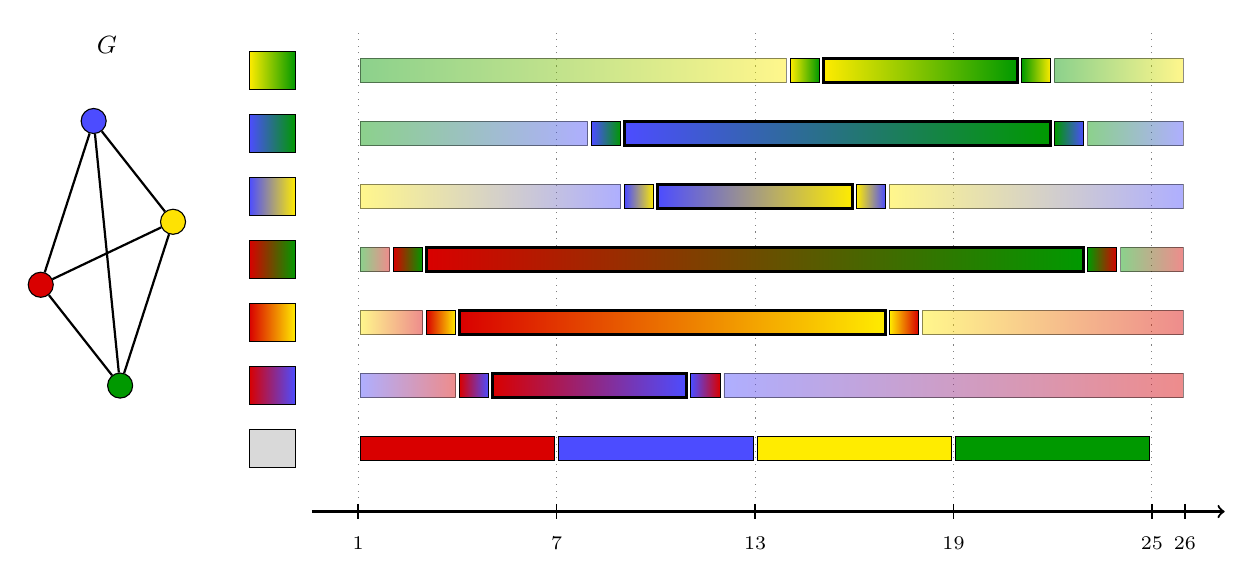
\begin{tikzpicture}[xscale=0.42,yscale=0.8]
  \colorlet{c0}{red!85!black}
  \colorlet{c1}{blue!70!white}
  \colorlet{c2}{yellow!85!orange}
  \colorlet{c3}{green!60!black}
  \def\hh{0.19}
  \def\g{0.06}
  % \jobbar[outline options]{x1}{x2}{y}{left color}{right color}
  \newcommand{\jobbar}[6][]{%
    \shade[left color=#5,right color=#6] (#2,#4-\hh) rectangle (#3,#4+\hh);
    \draw[line width=0.35pt,#1] (#2,#4-\hh) rectangle (#3,#4+\hh);}

  % the graph
  \node[circle,draw,fill=c0,inner sep=3.2pt] (v0) at (-8.6,3.6) {};
  \node[circle,draw,fill=c1,inner sep=3.2pt] (v1) at (-7.0,6.2) {};
  \node[circle,draw,fill=c2,inner sep=3.2pt] (v2) at (-4.6,4.6) {};
  \node[circle,draw,fill=c3,inner sep=3.2pt] (v3) at (-6.2,2.0) {};
  \foreach \s/\t in {v0/v1,v0/v2,v0/v3,v1/v2,v1/v3,v2/v3} \draw[line width=0.8pt] (\s) -- (\t);
  \node at (-6.6,7.4) {\small $G$};

  % time axis and the four vertex windows
  \foreach \x in {1,7,13,19,25}
    \draw[line width=0.4pt,dotted,gray] (\x,0) -- (\x,7.6);
  \draw[line width=0.8pt,->] (-0.4,0) -- (27.2,0);
  \foreach \x in {1,7,13,19,25,26}{
    \draw[line width=0.6pt] (\x,0.12) -- (\x,-0.12);
    \node at (\x,-0.5) {\scriptsize \x};}

  % validation machine: the vertex job of each vertex for its own color
  \draw[fill=gray!30,line width=0.35pt] (-2.3,1-0.3) rectangle (-0.9,1+0.3);
  \foreach \c in {0,...,3}{
    \pgfmathsetmacro{\xa}{6*\c+1+\g}
    \pgfmathsetmacro{\xb}{6*\c+7-\g}
    \jobbar{\xa}{\xb}{1}{c\c}{c\c}}

  % one edge selection machine per color combination
  \foreach \a/\b/\row in {0/1/1,0/2/2,0/3/3,1/2/4,1/3/5,2/3/6}{
    \pgfmathsetmacro{\y}{1+\row}
    \pgfmathsetmacro{\su}{6*(\a+1)-\b-1}
    \pgfmathsetmacro{\sv}{6*(\b+1)-\a-1}
    \shade[left color=c\a,right color=c\b] (-2.3,\y-0.3) rectangle (-0.9,\y+0.3);
    \draw[line width=0.35pt] (-2.3,\y-0.3) rectangle (-0.9,\y+0.3);
    \begin{scope}[opacity=0.45]
      \jobbar{1+\g}{\su-\g}{\y}{c\b}{c\a}
      \jobbar{\sv+1+\g}{26-\g}{\y}{c\b}{c\a}
    \end{scope}
    \jobbar{\su+\g}{\su+1-\g}{\y}{c\a}{c\b}
    \jobbar{\sv+\g}{\sv+1-\g}{\y}{c\b}{c\a}
    \jobbar[line width=1.1pt]{\su+1+\g}{\sv-\g}{\y}{c\a}{c\b}}
\end{tikzpicture}

    \caption{\Cref{const:w1hard} for a clique on $k=4$ colors, drawn to scale, with the
    schedule of weight $W$. Each row is a machine: the validation machine (gray) processes
    the vertex job $j_v^{(\ell)}$ of every vertex, and the edge selection machine of each
    color combination processes a color combination job (pale), a unit vertex job, the edge
    job (bold), a unit vertex job and a color combination job.}
    \label{fig:w1_overview}
\end{figure}

% lax begin Lax470956Proofs.Construction1Renum.correct
\begin{lemma}[Lemmas~1 and~2 of~\cite{HIMS24}]\label{lem:corr1}
Let $I$ be the \ProbEM\ instance computed from $G$ as specified by \Cref{const:w1hard}.
Then $G$ contains a clique of size $k$ if and only if there is a feasible schedule
$\sigma$ for $I$ with $w(\sigma)\ge W$.
\end{lemma}
\begin{proof}[Proof idea]
Given a clique, schedule on the edge selection machine for $\ell,\ell'$ the edge job of the
clique edge between $V_\ell$ and $V_{\ell'}$ together with the four jobs around it, and
schedule the vertex jobs $j_v^{(\ell)}$ of the clique vertices and all vertex jobs of the
other vertices with weight $c_1$ on the validation machine. Conversely, a schedule of
weight $W$ must schedule exactly one edge job on every edge selection machine, since $c_3$
exceeds the total weight of all other jobs. The weights $c_2$ force the two color
combination jobs next to it to belong to its endpoints, and the weights $c_1$ force the
$\binom{k}{2}$ selected edges to agree on one vertex per color.
\end{proof}
% lax end

% lax begin Lax470956.Theorem1
\begin{theorem}\label{thm:w1hard}
\MCC\ parameterized by the number $k$ of colors has a parameterized reduction to \ProbEM\
parameterized by the number $m$ of machines. The reduction is \Cref{const:w1hard}, and it
produces $m=\binom{k}{2}+1$ machines.
\end{theorem}
% lax end
Since \MCC\ is \Wone-hard, \ProbEM\ is \Wone-hard when parameterized by $m$. The class
\Wone\ is not formalized; the formalized statement is the reduction.

\section{\textsf{NP}-hardness for constant \texorpdfstring{$\boldsymbol{\pmax}$}{pmax}}\label{sec:nph}

% lax begin Lax470956.SatVariant
\begin{definition}[\SAT]
We are given a Boolean formula $\phi$ in conjunctive normal form where every clause has
exactly three literals and every variable appears at most four times, and are asked
whether $\phi$ has a satisfying assignment.
\end{definition}
\SAT\ is \NP-hard~\cite{Tovey84}.
% lax end
% lax begin Lax470956.Exact34Encoding
For the reduction, $\phi$ is given as a word that lists, for the $h$th literal of each
clause, its variable, whether it is negated, and which appearance of its variable it is.
% lax end

% lax begin Lax470956.Construction2
\begin{construction}\label{const:nph}
Let $\phi$ be a formula as above. We construct an instance $I$ of \ProbEM\ as follows.
\begin{itemize}
\item For each variable $x$ we create two machines $i_x^T,i_x^F$ and one job $j_x$ with
  deadline and processing time $25$ that is eligible on $i_x^T$ and $i_x^F$.
\item For each clause $c$ we create three machines $i_c^{(1)},i_c^{(2)},i_c^{(3)}$ and
  nine jobs.
\item Three of them are \emph{literal jobs} $j_c^{(1)},j_c^{(2)},j_c^{(3)}$ with
  processing time one. Let the $h$th literal of $c$ be the $k$th appearance of variable
  $x$. Then the deadline of $j_c^{(h)}$ is $2k+8h-8$. It is eligible on
  $i_c^{(2)},i_c^{(3)}$, and on $i_x^T$ if $x$ appears non-negated and on $i_x^F$
  otherwise.
\item For each literal job $j_c^{(h)}$ with deadline $d$ we create two \emph{wrapper
  jobs}: $j_{c,\alpha}^{(h)}$ with deadline and processing time $d-1$, and
  $j_{c,\omega}^{(h)}$ with deadline $25$ and processing time $25-d$. All wrapper jobs are
  eligible on $i_c^{(1)},i_c^{(2)},i_c^{(3)}$.
\end{itemize}
All jobs have weight one. See \Cref{fig:pmax} for an illustration.
\end{construction}
% lax end

\begin{figure}[tb]
    \centering
    % Construction 2 on the clause c = (x or y or not z), drawn to scale.
% Adapted from the slide "Reduction from Exact (3,4)-SAT" and Figure 3 of the paper.
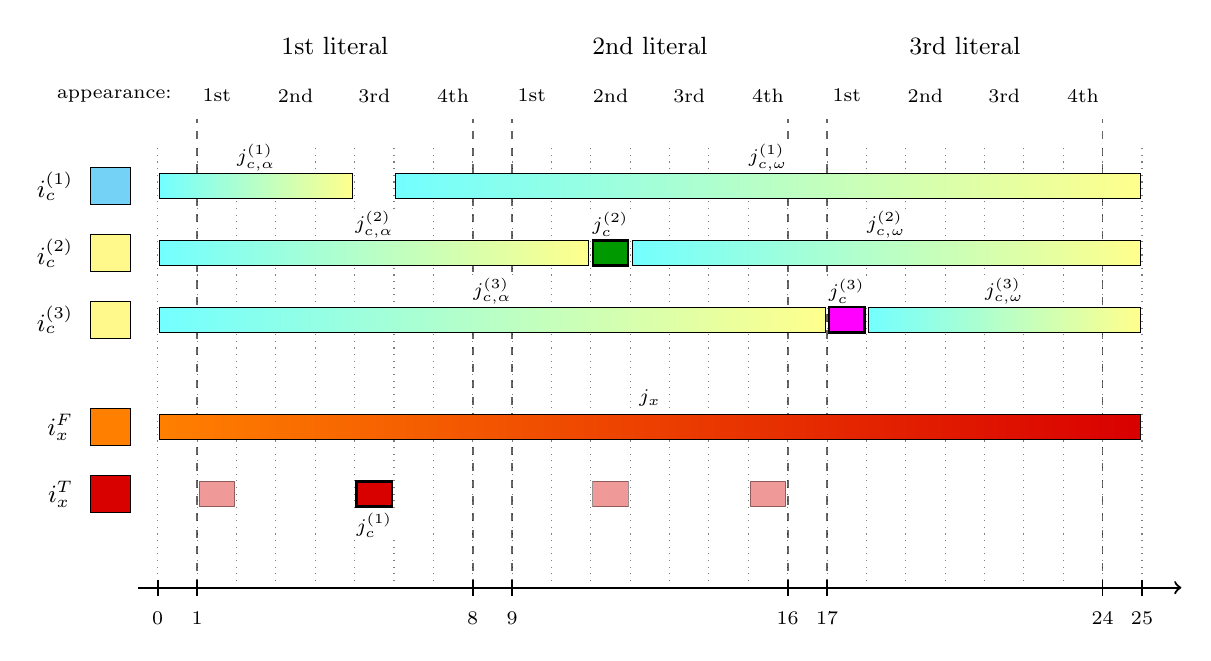
\begin{tikzpicture}[xscale=0.5,yscale=0.85]
  \colorlet{wa}{cyan!55}
  \colorlet{wb}{yellow!45}
  \colorlet{lx}{red!85!black}
  \colorlet{ly}{green!60!black}
  \colorlet{lz}{magenta}
  \def\hh{0.19}
  \def\g{0.05}
  \newcommand{\jobbar}[6][]{%
    \shade[left color=#5,right color=#6] (#2,#4-\hh) rectangle (#3,#4+\hh);
    \draw[line width=0.35pt,#1] (#2,#4-\hh) rectangle (#3,#4+\hh);}
  \newcommand{\machine}[3]{% y, color, label
    \draw[fill=#2,line width=0.35pt] (-1.7,#1-0.28) rectangle (-0.7,#1+0.28);
    \node[anchor=east] at (-1.9,#1) {\small #3};}

  % slots
  \foreach \i in {0,...,25}
    \draw[line width=0.4pt,dotted,opacity=0.5] (\i,0) -- (\i,6.6);
  \foreach \i in {1,8,9,16,17,24}
    \draw[line width=0.6pt,dashed,opacity=0.6] (\i,0) -- (\i,7.0);
  \draw[line width=0.8pt,->] (-0.5,0) -- (26,0);
  \foreach \i in {0,1,8,9,16,17,24,25}{
    \draw[line width=0.6pt] (\i,0.12) -- (\i,-0.12);
    \node at (\i,-0.45) {\scriptsize \i};}
  \foreach \h/\lab in {1/1st,2/2nd,3/3rd}{
    \node at (8*\h-3.5,8.1) {\small \lab\ literal};
    \foreach \k/\klab in {1/1st,2/2nd,3/3rd,4/4th}
      \node[fill=white,inner sep=0.8pt] at (2*\k+8*\h-8.5,7.35) {\scriptsize \klab};}
  \node[anchor=east] at (0.6,7.35) {\scriptsize appearance:};

  % the three machines of the clause
  \machine{6}{wa}{$i_c^{(1)}$}
  \machine{5}{wb}{$i_c^{(2)}$}
  \machine{4}{wb}{$i_c^{(3)}$}
  \jobbar{0+\g}{5-\g}{6}{wa}{wb}   \node[fill=white,inner sep=0.8pt] at (2.5,6.43) {\scriptsize $j^{(1)}_{c,\alpha}$};
  \jobbar{6+\g}{25-\g}{6}{wa}{wb}  \node[fill=white,inner sep=0.8pt] at (15.5,6.43) {\scriptsize $j^{(1)}_{c,\omega}$};
  \jobbar{0+\g}{11-\g}{5}{wa}{wb}  \node[fill=white,inner sep=0.8pt] at (5.5,5.43) {\scriptsize $j^{(2)}_{c,\alpha}$};
  \jobbar[line width=0.9pt]{11+\g}{12-\g}{5}{ly}{ly} \node[fill=white,inner sep=0.8pt] at (11.5,5.43) {\scriptsize $j^{(2)}_{c}$};
  \jobbar{12+\g}{25-\g}{5}{wa}{wb} \node[fill=white,inner sep=0.8pt] at (18.5,5.43) {\scriptsize $j^{(2)}_{c,\omega}$};
  \jobbar{0+\g}{17-\g}{4}{wa}{wb}  \node[fill=white,inner sep=0.8pt] at (8.5,4.43) {\scriptsize $j^{(3)}_{c,\alpha}$};
  \jobbar[line width=0.9pt]{17+\g}{18-\g}{4}{lz}{lz} \node[fill=white,inner sep=0.8pt] at (17.5,4.43) {\scriptsize $j^{(3)}_{c}$};
  \jobbar{18+\g}{25-\g}{4}{wa}{wb} \node[fill=white,inner sep=0.8pt] at (21.5,4.43) {\scriptsize $j^{(3)}_{c,\omega}$};

  % the two machines of the variable x
  \machine{2.4}{orange}{$i_x^{F}$}
  \machine{1.4}{lx}{$i_x^{T}$}
  \jobbar{0+\g}{25-\g}{2.4}{orange}{lx} \node[fill=white,inner sep=0.8pt] at (12.5,2.83) {\scriptsize $j_x$};
  \begin{scope}[opacity=0.4]
    \foreach \s in {1,11,15} {\jobbar{\s+\g}{\s+1-\g}{1.4}{lx}{lx}}
  \end{scope}
  \jobbar[line width=0.9pt]{5+\g}{6-\g}{1.4}{lx}{lx} \node[fill=white,inner sep=0.8pt] at (5.5,0.93) {\scriptsize $j^{(1)}_{c}$};
\end{tikzpicture}

    \caption{\Cref{const:nph} applied to the clause $c=(x\vee y\vee\neg z)$, which contains
    the third appearance of $x$, the second appearance of $y$, and the first appearance of
    $z$. The dashed lines delimit the slots of the literal jobs. Shown is a schedule for an
    assignment that sets $x$ to true: $j_x$ is on $i_x^F$, the literal job $j_c^{(1)}$ is
    on $i_x^T$ together with the literal jobs of other appearances of $x$ (pale), and its
    two wrapper jobs are on $i_c^{(1)}$.}
    \label{fig:pmax}
\end{figure}

% lax begin Lax470956Proofs.Construction2.correct
\begin{lemma}[Lemmas~3 and~4 of~\cite{HIMS24}]\label{lem:nphcorr}
Let $I$ be the \ProbEM\ instance computed from $\phi$ as specified by \Cref{const:nph}.
Then $\phi$ is satisfiable if and only if there is a feasible schedule for $I$ such that
all jobs are scheduled.
\end{lemma}
\begin{proof}[Proof idea]
Job $j_x$ blocks one of $i_x^T,i_x^F$ for the whole time; we set $x$ to true if and only if
$j_x$ is scheduled on $i_x^F$. In a schedule of all jobs the two wrapper jobs of each
literal job are on the same machine, so the machines $i_c^{(2)},i_c^{(3)}$ have room for
two of the three literal jobs of $c$, and the third one is scheduled on a machine of its
variable, which makes its literal true. Distinct appearances of a variable have
non-overlapping literal jobs, so a satisfying assignment yields a schedule of all jobs.
\end{proof}
% lax end

% lax begin Lax470956.Theorem2
\begin{theorem}\label{thm:nph}
It is \NP-hard to decide whether all jobs of a \ProbEM\ instance can be scheduled, even
when $\pmax\le 25$ and all jobs have unit weight.
\end{theorem}
% lax end

\section{\textsf{FPT} for the combination of \texorpdfstring{$\boldsymbol{m}$ and $\boldsymbol{\pmax}$}{m and pmax}}\label{sec:FPTalt}

% lax begin Lax470956.Preprocessing
\begin{construction}\label{con:effective}
Let $I$ be an instance of \ProbEM. For every interval $[r,d)$ and every machine $i$ let
$S^{(i)}_{[r,d)}$ denote the set of the $m$ highest-weighted jobs that have interval
$[r,d)$ and are eligible on machine $i$, where ties are broken by the index of the job. All
jobs that are not contained in any set $S^{(i)}_{[r,d)}$ are discarded.
\end{construction}
% lax begin Lax470956Proofs.Preprocessing.optimumOn_keep
\begin{lemma}[Lemma~5 of~\cite{HIMS24}]\label{lem:EM2EM}
Let $I'$ be obtained from $I$ by applying \Cref{con:effective}. Then the maximum weight of
a feasible schedule is the same for $I$ and $I'$.
\end{lemma}
% lax end
% lax begin Lax470956Proofs.Preprocessing.card_keep_alive_le
\begin{observation}[Observation~5 of~\cite{HIMS24}]\label{obs:fpt}
Let $I'$ be obtained from $I$ by applying \Cref{con:effective}. Then for every time step
$t$ there are at most $m^2\pmax^2$ jobs in $I'$ whose interval contains $t$.
\end{observation}
% lax end
% lax end

\begin{figure}[tb]
    \centering
    % The intervals of length at most p_max that contain a time step t.
% Adapted from the slide "Data Reduction Procedure" and Figure 4 of the paper.
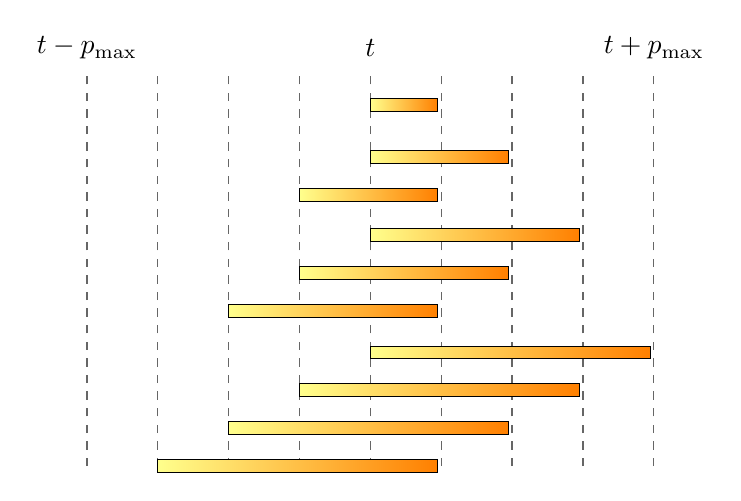
\begin{tikzpicture}[scale=0.9]
\def\dy{3}
\def\barh{0.09}
\foreach \x in {-4,...,4}
    \draw[line width=0.5pt, dashed, opacity=0.6] (\x,-5.3) -- (\x,0.25);
\node at (-4,0.6) {$t-\pmax$};
\node at (0,0.6) {$t$};
\node at (4,0.6) {$t+\pmax$};
\foreach \i/\p in {1/1,2/2,3/3,4/4}
{
    \pgfmathtruncatemacro{\pstar}{\p - 1}
    \foreach \r in {-\pstar,...,0}
    {
        \pgfmathsetmacro{\y}{\r/\dy - \i*.85*\i/\dy + \i/\dy+\r*.2+.25/(\i*\i*\i)-.5}
        \pgfmathsetmacro{\xend}{\r+\p-0.05}
        \shade[left color=yellow!45, right color=orange] (\r,\y-\barh) rectangle (\xend,\y+\barh);
        \draw[line width=0.35pt] (\r,\y-\barh) rectangle (\xend,\y+\barh);
    }
}
\end{tikzpicture}

    \caption{There are at most $\pmax^2$ distinct intervals of length at most $\pmax$ that
    contain time step $t$.}
    \label{fig:m2p2-interval}
\end{figure}

% lax begin Lax470956.DynamicProgram
For a time step $t$ let $J_t$ be the set of jobs whose interval contains $t$. The dynamic
programming table $T_t:(J_t\cup\{\bot\})^m\to\mathbb{N}$ is defined as follows: the entry
$T_t[\ell_1,\ldots,\ell_m]$ is the maximum weight of the scheduled jobs that start at or
before $t$, over all feasible schedules such that for each $i\in\{1,\ldots,m\}$, at time
$t$ machine $i$ processes job $\ell_i$ if $\ell_i\neq\bot$ and is idle if $\ell_i=\bot$. An
entry is \emph{valid} if $i\in M_{\ell_i}$ for all $i$ with $\ell_i\neq\bot$ and no job
appears twice. For a valid entry, $T_0[\ell_1,\ldots,\ell_m]$ is the total weight of the
jobs $\ell_1,\ldots,\ell_m$, and
\[
T_{t+1}[\ell'_1,\ldots,\ell'_m]=\max_{[\ell_1,\ldots,\ell_m]\to[\ell'_1,\ldots,\ell'_m]}
T_t[\ell_1,\ldots,\ell_m]\;+\sum_{\substack{j\in\{\ell'_1,\ldots,\ell'_m\}\\ d_j-p_j=t+1}}w_j,
\]
where the maximum is over the valid entries of $T_t$ such that every job $\ell_i$ that is
still processed at time $t+1$ satisfies $\ell'_i=\ell_i$, and every job $\ell'_i$ that
starts at or before $t$ satisfies $\ell_i=\ell'_i$. The table $T_t$ has at most
$(|J_t|+1)^m$ entries.
% lax begin Lax470956Proofs.DynamicProgram.dp_eq_optAt
\begin{lemma}[Lemma~6 of~\cite{HIMS24}]\label{lem:dpcorrectness2}
The recursion above correctly computes $T_t[\ell_1,\ldots,\ell_m]$ for every time step $t$
and every valid entry. In particular, for $D=\max_j d_j$ the entry
$T_D[\bot,\ldots,\bot]$ is the maximum weight of a feasible schedule.
\end{lemma}
% lax end
% lax end

% lax begin Lax470956.Theorem3
\begin{theorem}\label{thm:fpt}
There are a word RAM program and a constant $c$ such that for every instance $x$ of
\ProbEM\ with target weight $W$ that fits into words, the program decides whether there is
a feasible schedule $\sigma$ with $w(\sigma)\ge W$ within
\[
c\cdot(m\cdot\pmax+1)^{2m}\cdot(m+1)\cdot(|x|+1)
\]
instructions. Hence \ProbEM\ is fixed-parameter tractable when parameterized by $m+\pmax$.
\end{theorem}
% lax end
This is the running time $\bigO((m\cdot\pmax)^{2m}\cdot mn)$ of~\cite{HIMS24} with explicit
constants: by \Cref{obs:fpt} we have $|J_t|\le m^2\pmax^2$ after applying
\Cref{con:effective}, so every table has at most $(m\cdot\pmax+1)^{2m}$ entries.

\begin{thebibliography}{9}
\bibitem{AS87}
E.~M. Arkin and E.~B. Silverberg.
\newblock Scheduling jobs with fixed start and end times.
\newblock \emph{Discrete Applied Mathematics} 18(1):1--8, 1987.
\newblock \doi{10.1016/0166-218X(87)90037-0}
\bibitem{FHRV09}
M.~R. Fellows, D.~Hermelin, F.~Rosamond and S.~Vialette.
\newblock On the parameterized complexity of multiple-interval graph problems.
\newblock \emph{Theoretical Computer Science} 410(1):53--61, 2009.
\newblock \doi{10.1016/j.tcs.2008.09.065}
\bibitem{HIMS24}
D.~Hermelin, Y.~Itzhaki, H.~Molter and D.~Shabtay.
\newblock On the parameterized complexity of interval scheduling with eligible machine sets.
\newblock \emph{Journal of Computer and System Sciences} 144:103533, 2024.
\newblock \doi{10.1016/j.jcss.2024.103533}
\bibitem{MvB18}
M.~Mnich and R.~van Bevern.
\newblock Parameterized complexity of machine scheduling: 15 open problems.
\newblock \emph{Computers \& Operations Research} 100:254--261, 2018.
\newblock \doi{10.1016/j.cor.2018.07.020}
\bibitem{Tovey84}
C.~A. Tovey.
\newblock A simplified NP-complete satisfiability problem.
\newblock \emph{Discrete Applied Mathematics} 8(1):85--89, 1984.
\newblock \doi{10.1016/0166-218X(84)90081-7}
\end{thebibliography}

\end{document}
